\documentclass{article}

\usepackage{Sweave}
\begin{document}
\Sconcordance{concordance:test.tex:test.Rnw:%
1 2 1 1 0 4 1 1 2 1 0 2 1 4 0 1 2 2 1 1 2 8 0 1 2 2 1 1 2 5 0 1 2 2 1 1 %
2 1 0 1 1 4 0 1 2 3 1}


Let me create some random data:

\begin{Schunk}
\begin{Sinput}
> set.seed(457299)
> x=rnorm(100,10,3)
> boxplot(x)
\end{Sinput}
\end{Schunk}
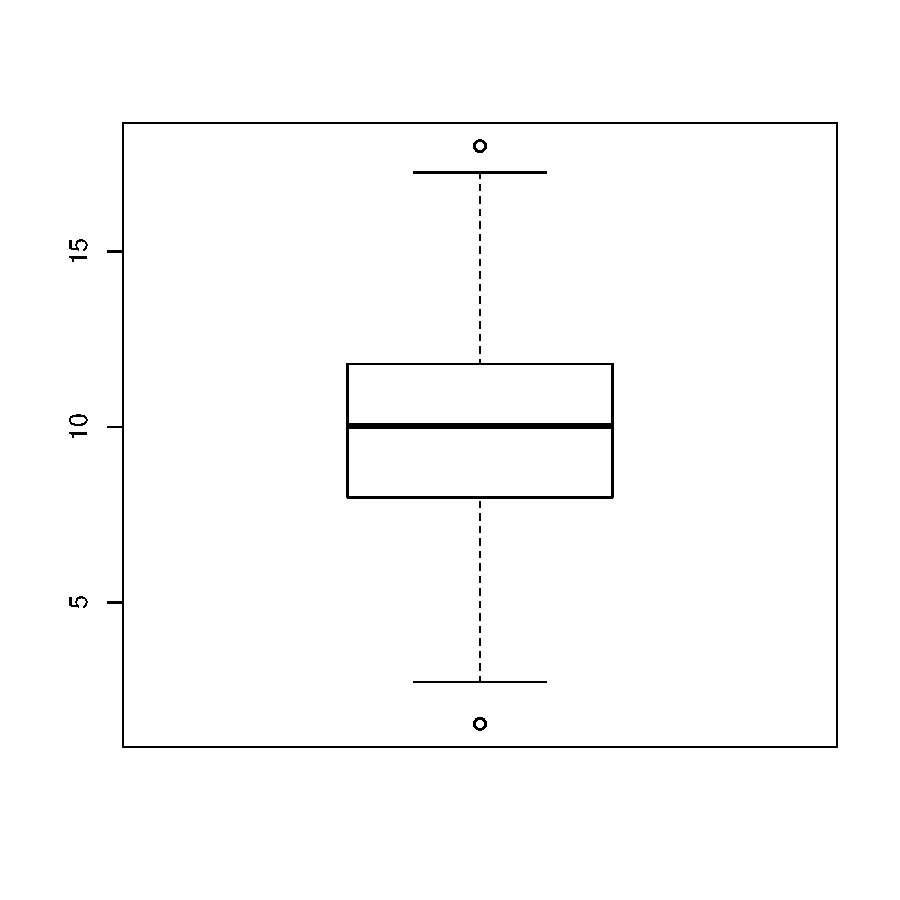
\includegraphics{test-001}

This is normal data, so we're not expecting any serious outliers. The boxplot reveals two small outliers, one at each end. A summary of \texttt{x} looks like this:

\begin{Schunk}
\begin{Sinput}
> summary(x)
\end{Sinput}
\begin{Soutput}
   Min. 1st Qu.  Median    Mean 3rd Qu.    Max. 
  1.536   8.026  10.030   9.930  11.780  18.010 
\end{Soutput}
\end{Schunk}

These data were generated from a normal distribution, but how normal do they look? One answer is to get a histogram:

\begin{Schunk}
\begin{Sinput}
> hist(x)
\end{Sinput}
\end{Schunk}
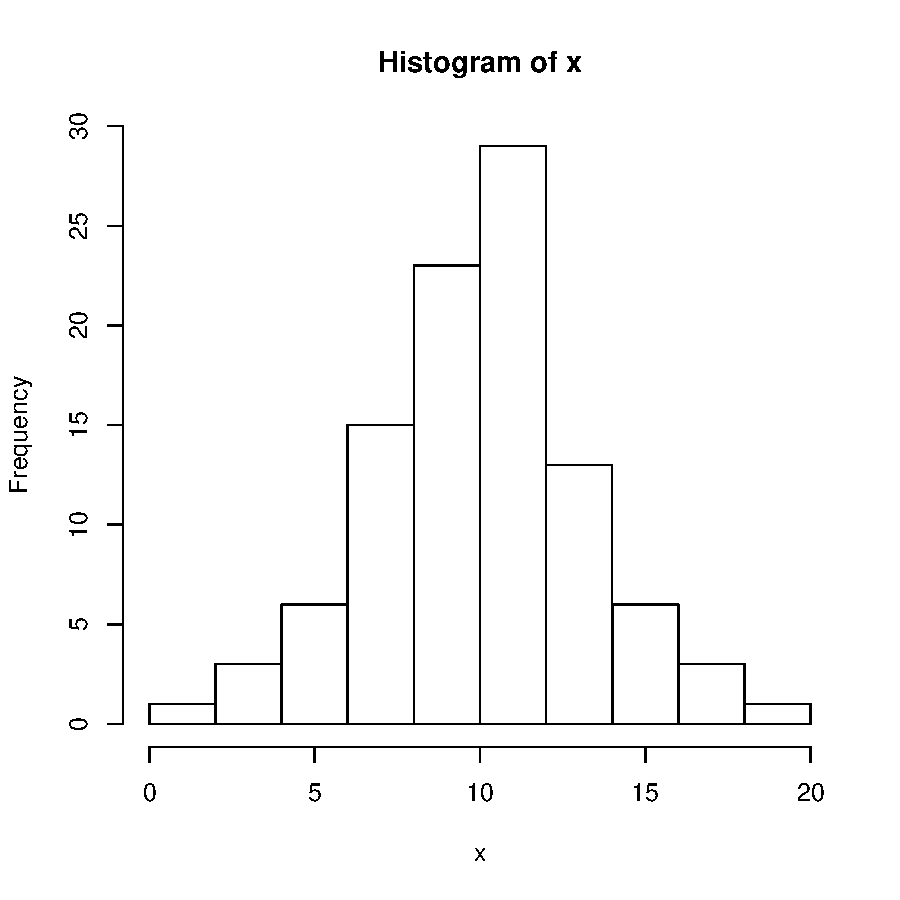
\includegraphics{test-003}

and another is a normal quantile plot:

\begin{Schunk}
\begin{Sinput}
> qqnorm(x)
> qqline(x)
\end{Sinput}
\end{Schunk}
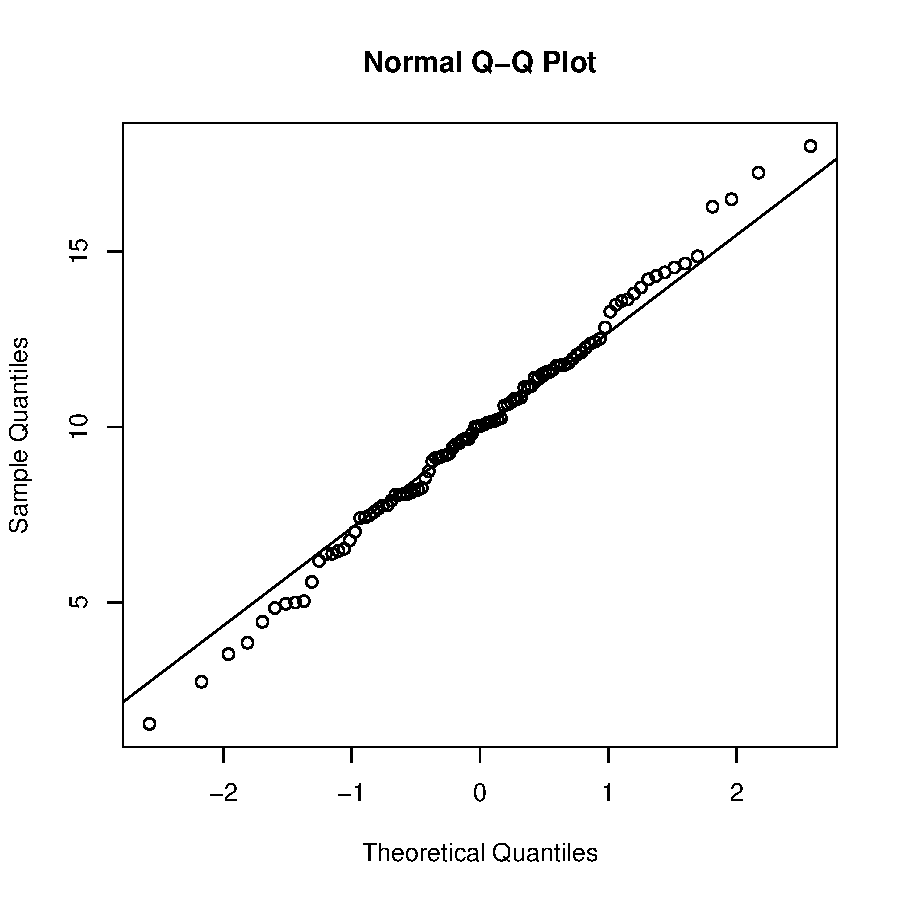
\includegraphics{test-004}

These both look pretty normal, so the suggestion is that those outliers on the boxplot are not to be taken seriously.

\end{document}
